%%%%%%%%%%%%%%%%%%%%%%%%%
%%  Capítulo 3: Principios de reflectores parabólicos  %%
%%%%%%%%%%%%%%%%%%%%%%%%%

%%%%
\section{Introducción}
\label{sec_principios_intro}
%%%%

%%%%
Lo que comúnmente se conoce como antena parabólica está en realidad compuesto por dos elementos: la antena propiamente dicha, que cumple la función de iluminador o alimentador, y la superficie reflectora, que consiste en un paraboloide de revolución.
%%%%
\begin{figure}[H]
\centering
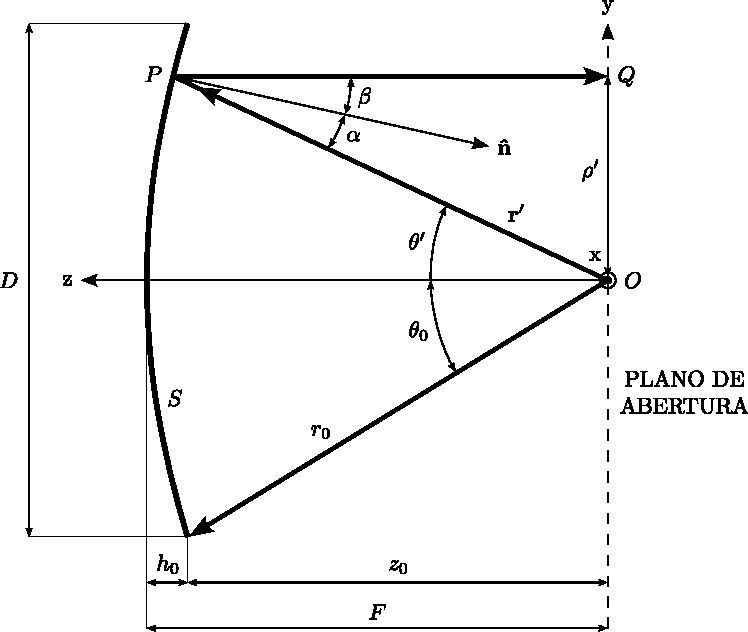
\includegraphics[scale = 0.97]{Figures/Principios/principios_1}
\caption{Esquema bidimensional de un reflector parabólico.}
\label{fig_principios:1}
\end{figure}
%%%%
En la figura \ref{fig_principios:1} puede observarse un esquema bidimensional de un reflector parabólico. La ecuación que describe la curva parabólica resultante de la intersección entre el paraboloide de revolución y cualquier plano que contenga al eje \emph{z}, en función de la distancia focal $F$, es:
%%%%
\begin{align}
{\rho '}^2 = 4F\left(F - z'\right),\hspace{5mm}\rho '\leq\frac{D}{2}
\label{ec_principios:1}
\end{align}
%%%%
Para un desplazamiento dado $\rho '$ desde el eje del reflector, $r'$ es la distancia entre el punto $P$ sobre la superficie del reflector y el punto focal $O$. La curva parabólica puede expresarse también en coordenadas polares como:
%%%%
\begin{align}
r' = \frac{2F}{1 + \cos\theta '} = F\sec^2\left(\frac{\theta '}{2}\right)
\label{ec_principios:2}
\end{align}
%%%%
y la proyección de $r'$ sobre el plano de abertura es:
%%%%
\begin{align}
\rho ' = r'\sen\theta ' = \frac{2F\sen\theta '}{1 + \cos\theta '} = 2F\tan\left(\frac{\theta '}{2}\right)
\label{ec_principios:3}
\end{align}
%%%%
Comúnmente, la curvatura del reflector se expresa en términos de $F/D$ y $\theta_0$, donde $F/D$ es la \emph{relación distancia focal-diámetro} y $\theta_0$ es el \emph{ángulo de abertura máximo}, formado entre el punto focal $O$ y el borde del reflector. A partir de la figura \ref{fig_principios:1} puede determinarse la relación entre $F/D$ y $\theta_0$, cuya expresión resulta:
%%%%
\begin{align}
\dfrac{F}{D} = \frac{1}{4}\cot\left(\frac{\theta_0}{2}\right)
\label{ec_principios:4}
\end{align}
%%%%
y su gráfica puede observarse en la figura \ref{fig_principios:2}.
%%%%
\begin{figure}[H]
\begin{minipage}{.5\textwidth}
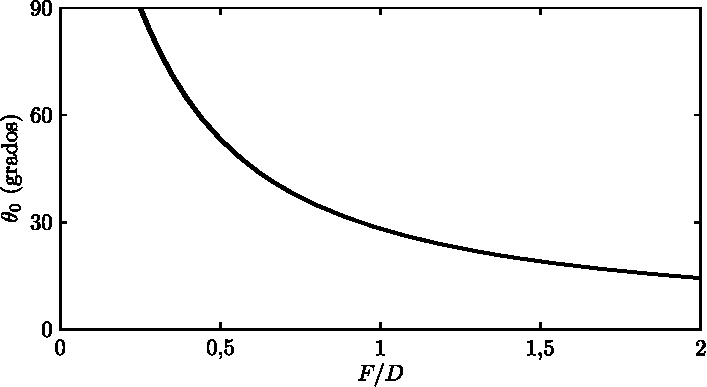
\includegraphics[scale = 1]{Figures/Principios/principios_2}
\end{minipage}
\begin{minipage}{.5\textwidth}
\hfill
\begin{tabular}{cc}
$F/D$ & $\theta_0$ \\
\hline
0,25 & 90,0$^{\circ}$\\
0,30 & 79,6$^{\circ}$\\
0,33 & 73,7$^{\circ}$\\
0,40 & 64,0$^{\circ}$\\
0,50 & 53,1$^{\circ}$\\
1,00 & 28,1$^{\circ}$\\
\\
\end{tabular}
\end{minipage}
\caption{Angulo $\theta_0$ en función de $F/D$.}
\label{fig_principios:2}
\end{figure}
%%%%
A partir de la óptica geométrica (GO) surgen las siguientes propiedades de gran importancia de los reflectores parabólicos:
\begin{enumerate}
\item Los rayos que emergen del punto focal $O$ se coliman luego de reflejarse en la superficie metálica del reflector, y los rayos reflejados son paralelos al eje del reflector (eje \emph{z}).
\item La longitud de todos los caminos que describen los rayos desde el punto focal $O$ hasta el plano de abertura, luego de reflejarse en la superficie metálica del reflector, es la misma e igual a $2F$.
\end{enumerate}
%%%%
La primera propiedad se dedude directamente de la aplicación de la ley de reflexión de Snell en la superficie del reflector, o sea, tomando que $\alpha = \beta$. Para demostrar esto, primero se determina la superficie normal al punto de reflexión $P$ evaluando el gradiente de la ecuación de la curva parabólica $S = F - r'\cos^2\left(\theta '/2\right) = 0$, basada en la expresión \eqref{ec_principios:2}; entonces:
%%%%
\begin{align}
\begin{split}
\mathbf{N} &= \nabla S = \nabla\left[f - r'\cos^2\left(\frac{\theta '}{2}\right)\right] = \left(\frac{\partial S}{\partial r'}\versor{r}' + \frac{1}{r'}\frac{\partial S}{\partial\theta '}\versor{\uptheta}'\right)\\
&= -\cos^2\left(\frac{\theta '}{2}\right)\!\versor{r}' + \cos\left(\frac{\theta '}{2}\right)\sen\left(\frac{\theta '}{2}\right)\!\versor{\uptheta}'
\end{split}
\label{ec_principios:5}
\end{align}
%%%%
Se halla la expresión del vector unitario $\versor{n}$ utilizando $|\mathbf{N}| = \cos^2\left(\dfrac{\theta '}{2}\right)$, obteniendo:
%%%%
\begin{align}
\versor{n} = \frac{\mathbf{N}}{|\mathbf{N}|} = -\cos\left(\frac{\theta '}{2}\right)\!\versor{r}' + \sen\left(\frac{\theta '}{2}\right)\!\versor{\uptheta}'
\label{ec_principios:6}
\end{align}
%%%%
Para hallar el ángulo formado entre el vector unitario $\versor{n}$, que es normal a la superficie $\mathbf{N}$ en el punto de reflexión $P$, y la onda incidente, se formula:
%%%%
\begin{align}
\cos\alpha = -\versor{r}'\prodesc\versor{n} = -\versor{r}'\prodesc\left[-\cos\left(\frac{\theta '}{2}\right)\!\versor{r}' + \sen\left(\frac{\theta '}{2}\right)\!\versor{\uptheta}'\right] = \cos\left(\frac{\theta '}{2}\right)
\label{ec_principios:7}
\end{align}
%%%%
Procediendo análogamente para hallar el ángulo formado entre el vector unitario $\versor{n}$ y la onda reflejada:
%%%%
\begin{align}
\begin{split}
\cos\beta &= -\versor{z}'\prodesc\versor{n} = -\versor{z}'\prodesc\left[-\cos\left(\frac{\theta '}{2}\right)\!\versor{r}' + \sen\left(\frac{\theta '}{2}\right)\!\versor{\uptheta}'\right]\\
&= -\left(\cos\theta '\,\versor{r}' - \sen\theta '\,\versor{\uptheta}'\right)\prodesc\left[-\cos\left(\frac{\theta '}{2}\right)\!\versor{r}' + \sen\left(\frac{\theta '}{2}\right)\!\versor{\uptheta}'\right] = \cos\left(\frac{\theta '}{2}\right)
\end{split}
\label{ec_principios:8}
\end{align}
%%%%
Comparando las expresiones \eqref{ec_principios:7} y \eqref{ec_principios:8}, puede observarse que:
%%%%
\begin{align}
\alpha = \beta = \frac{\theta '}{2}
\label{ec_principios:9}
\end{align}
%%%%
que es la expresión de la ley de reflexión de Snell. Como consecuencia de la primera propiedad, puede decirse que \emph{empleando un reflector parabólico, el frente de onda esférico radiado por una fuente ubicada en el foco emergerá a través del plano de abertura, luego de reflejarse en la superficie metálica del reflector, como un frente de onda plano}.

Para demostrar la segunda propiedad, a partir de la figura \ref{fig_principios:1} es posible expresar las distancias entre el punto focal $O$ y el punto de reflexión $P$ y entre $P$ y el punto sobre el plano de abertura $Q$ como:
%%%%
\begin{subequations}
\label{grup_ec_principios:1}
\begin{align}
\overline{OP} &= r'
\label{ec_principios:10}\\
\overline{PQ} &= r'\cos\theta
\label{ec_principios:11}
\end{align}
\end{subequations}
%%%%
y sumando ambas distancias se obtiene la longitud total del camino entre el foco y el plano de abertura luego de producirse la reflexión. Aplicando la expresión \eqref{ec_principios:2}, la longitud total queda expresada como:
%%%%
\begin{align}
\overline{OP} + \overline{PQ} = r' + r'\cos\theta ' = r'\left(1 + \cos\theta '\right) = 2F
\label{ec_principios:12}
\end{align}
%%%%
Dado que la longitud de los distintos caminos es constante e igual a $2F$, la fase de las ondas que arriben al plano de abertura desde un punto fuente ubicado en el foco también será constante. Por lo tanto, \emph{el reflector parabólico alimentado con una fuente que tenga el centro de fase en el foco generará una fase uniforme a través del plano de abertura}. Sin embargo, la distribución de amplitud en la abertura no será uniforme.

%%%%
\section{Campos radiados}
\label{sec_principios_cam_rad}
%%%%

%%%%
Para determinar las características de radiación de una antena parabólica, los dos métodos más empleados son:
\begin{itemize}
\item \emph{Método de distribución de campos sobre la abertura}: Se halla el campo reflejado sobre el plano de abertura empleando la óptica geométrica, quedando determinada una superficie circular que es la proyección del área del reflector que se denomina $S_0$, se forman las corrientes equivalentes sobre el plano de abertura, suponiendo que las fuentes son nulas fuera del área proyectada $S_0$, y luego se integran para hallar los campos radiados.
\item \emph{Método de distribución de corrientes}: Se determina la densidad de corriente inducida sobre la superficie iluminada del reflector ($S_1$ en la figura \ref{fig_principios:3}) empleando la óptica física (PO) y se hallan los campos radiados integrando la densidad de corriente inducida sobre $S_1$.
\end{itemize}
%%%%
\begin{figure}[H]
\centering
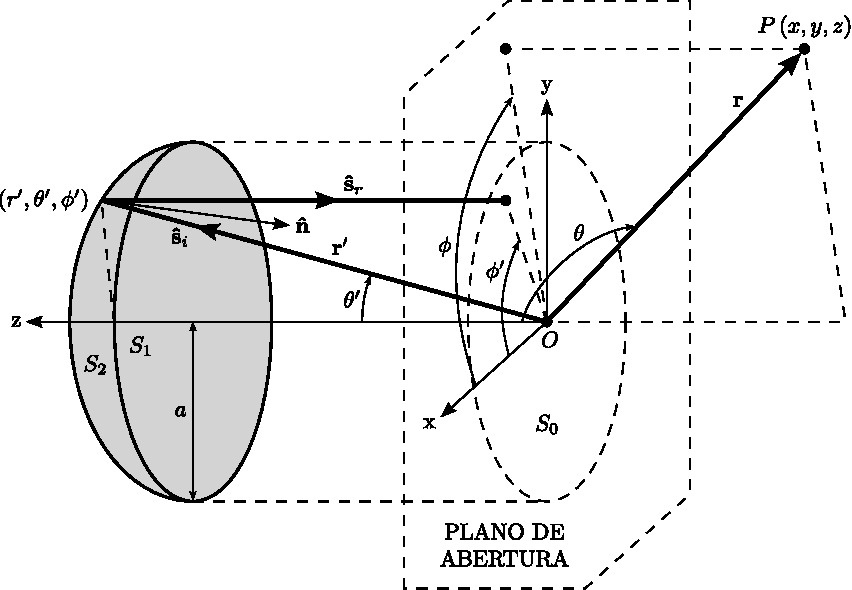
\includegraphics[scale = 1]{Figures/Principios/principios_3}
\caption{Geometría tridimensional de un reflector parabólico.}
\label{fig_principios:3}
\end{figure}
Si bien el método de distribución de campos sobre la abertura es más sencillo que el de distribución de corrientes, se emplea el segundo método debido a que se obtienen mejores aproximaciones.

Mediante la óptica física, se relaciona la densidad de corriente inducida con el campo incidente en la superficie del reflector. Previo a analizar el método, se consideran las siguientes aproximaciones:
%%%%
\begin{enumerate}
\item El reflector se comporta como un conductor perfecto, por lo que las amplitudes de las ondas incidente y reflejada son iguales; esto quiere decir que $\Gamma = -1$.
\item La densidad de corriente es nula en la superficie no iluminada del reflector ($S_2$ en la figura \ref{fig_principios:3}).
\item La discontinuidad de la densidad de corriente en el borde del reflector es despreciable.
\item La radiación directa del alimentador y el bloqueo parcial del haz emergente que éste produce son despreciables.
\end{enumerate}
%%%%
La densidad de corriente inducida $\mathbf{J}_s$ puede determinarse mediante:
%%%%
\begin{align}
\mathbf{J}_s = \versor{n}\prodvec\mathbf{H} = \versor{n}\prodvec\left(\mathbf{H}^i + \mathbf{H}^r\right)
\label{ec_principios:13}
\end{align}
%%%%
donde $\mathbf{H}^i$ y $\mathbf{H}^r$ representan, respectivamente, las componentes del campo magnético incidente y reflejado en la superficie del reflector. Considerando que la región del reflector localizada en torno a cada reflexión se trata como plana, aplicando teoría de imágenes:
%%%%
\begin{align}
\versor{n}\prodvec\mathbf{H}^i = \versor{n}\prodvec\mathbf{H}^r
\label{ec_principios:14}
\end{align}
%%%%
y la expresión \eqref{ec_principios:13} se reduce a:
%%%%
\begin{align}
\mathbf{J}_s = \versor{n}\prodvec\left(\mathbf{H}^i + \mathbf{H}^r\right) = 2\versor{n}\prodvec\mathbf{H}^i = 2\versor{n}\prodvec\mathbf{H}^r
\label{ec_principios:15}
\end{align}
%%%%
Si la superficie reflectora está, respecto al alimentador, en la zona de campo lejano, la expresión \eqref{ec_principios:15} resulta:
%%%%
\begin{align}
\mathbf{J}_s &= 2\versor{n}\prodvec\mathbf{H}^i \simeq \frac{2}{\eta}\left[\versor{n}\prodvec\left(\versor{s}_i\prodvec\mathbf{E}^i\right)\right]
\label{ec_principios:16}
\intertext{o también:}
\mathbf{J}_s &= 2\versor{n}\prodvec\mathbf{H}^r \simeq \frac{2}{\eta}\left[\versor{n}\prodvec\left(\versor{s}_r\prodvec\mathbf{E}^r\right)\right]
\tag{\ref{ec_principios:16}a}
\label{ec_principios:17}
\end{align}
%%%%
donde $\eta$ es la impedancia intrínseca del medio, $\versor{s}_i$ y $\versor{s}_r$ son los vectores unitarios a lo largo de los caminos de las ondas incidente y reflejada (como puede verse en la figura \ref{fig_principios:3}) y $\mathbf{E}^i$ y $\mathbf{E}^r$ son los campos eléctricos incidente y reflejado.

Suponiendo que una fuente polarizada linealmente en el eje \emph{y} con una ganancia $G_f\left(\theta ',\phi '\right)$ se ubica en el foco del reflector, su intensidad de radiación está dada por:
%%%%
\begin{align}
U\left(\theta ',\phi '\right) = \frac{P_t}{4\pi}G_f\left(\theta ',\phi '\right)
\label{ec_principios:18}
\end{align}
%%%%
donde $P_t$ es la potencia total radiada. Para campo lejano, se cumple que:
%%%%
\begin{align}
U\left(\theta ',\phi '\right) = {r'}^2\left<\mathbf{N}\right> = {r'}^2\frac{1}{2}\Re\left[\mathbf{E}\left(\theta ',\phi '\right)\prodvec\mathbf{H}^*\left(\theta ',\phi '\right)\right] = {r'}^2\frac{\left|\mathbf{E}\left(\theta ',\phi '\right)\right|^2}{2\eta}
\label{ec_principios:19}
\end{align}
%%%%
por lo que:
%%%%
\begin{align}
\left|\mathbf{E}\left(\theta ',\phi '\right)\right| = \sqrt{\frac{2\eta}{{r'}^2}U\left(\theta ',\phi '\right)} = \sqrt{\frac{\eta}{2\pi{r'}^2}P_tG_f\left(\theta ',\phi '\right)}
\label{ec_principios:20}
\end{align}
%%%%
El campo incidente puede expresarse como:
%%%%
\begin{gather}
\mathbf{E}^i\left(\theta ',\phi ', r'\right) = \sqrt{\eta\frac{P_t}{2\pi}G_f\left(\theta ',\phi '\right)}\,\frac{e^{-jkr'}}{r'}\,\versor{e}_i = C_1\sqrt{G_f\left(\theta ',\phi '\right)}\,\frac{e^{-jkr'}}{r'}\,\versor{e}_i
\label{ec_principios:21}\\
C_1 = \sqrt{\frac{\eta P_t}{2\pi}}
\tag{\ref{ec_principios:21}a}
\label{ec_principios:22}
\end{gather}
%%%%
donde $\versor{e}_i$ es un versor perpendicular a $\versor{r}'$ y paralelo al plano formado por $\versor{r}'$ y $\versor{y}$, como se muestra en la figura \ref{fig_principios:4}, que representa la polarización del campo incidente.
%%%%
\begin{figure}[H]
\centering
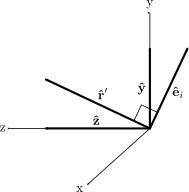
\includegraphics[scale = 1]{Figures/Principios/principios_4}
\caption{Sistema de alineación de vectores para un reflector parabólico.}
\label{fig_principios:4}
\end{figure}
%%%%
La expresión resultante de $\versor{e}_i$, desarrollada en el apéndice \ref{apendice_d}, es:
%%%%
\begin{align}
\versor{e}_i= -\dfrac{\sen^2\theta '\sen\phi '\cos\phi '}{\sqrt{1 - \sen^2\theta '\sen^2\phi '}}\versor{x} + \dfrac{\sen^2\theta '\cos^2\phi ' + \cos^2\theta'}{\sqrt{1 - \sen^2\theta '\sen^2\phi '}}\versor{y} - \dfrac{\sen\theta '\cos\theta '\sen\phi '}{\sqrt{1 - \sen^2\theta '\sen^2\phi '}}\versor{z}
\label{ec_principios:23}
\end{align}
%%%%
A partir de las expresiones \eqref{ec_principios:16} y \eqref{ec_principios:21}, puede demostrarse que en la superficie del reflector:
%%%%
\begin{gather}
\mathbf{J}_s = \dfrac{2}{\eta}\left[\versor{n}\prodvec\left(\versor{s}_i\prodvec\mathbf{E}^i\right)\right] = \dfrac{2}{\eta}\,C_1\sqrt{G_f\left(\theta ',\phi '\right)}\,\frac{e^{-jkr'}}{r'}\,\mathbf{u}
\label{ec_principios:24}\\
\mathbf{u} = \versor{n}\prodvec\left(\versor{r}'\prodvec\versor{e}_i\right) = \left(\versor{n}\prodesc\versor{e}_i\right)\versor{r}' - \left(\versor{n}\prodesc\versor{r}'\right)\versor{e}_i
\tag{\ref{ec_principios:23}a}
\label{ec_principios:25}
\end{gather}
%%%%
y el vector $\mathbf{u}$, cuya expresión fue deducida en el apéndice \ref{apendice_d}, resulta:
%%%%
\begin{align}
\begin{split}
\mathbf{u} &= -\dfrac{\sen\theta '\sen\left(\dfrac{\theta '}{2}\right)\sen\phi '\cos\phi '}{\sqrt{1 - \sen^2\theta '\sen^2\phi '}}\versor{x} + \dfrac{\cos\left(\dfrac{\theta '}{2}\right)\!\left(\cos\theta '\sen^2\phi ' + \cos^2\phi '\right)}{\sqrt{1 - \sen^2\theta '\sen^2\phi '}}\versor{y}\\
&-\dfrac{\cos\theta '\sen\left(\dfrac{\theta '}{2}\right)\sen\phi '}{\sqrt{1 - \sen^2\theta '\sen^2\phi '}}\versor{z}
\label{ec_principios:26}
\end{split}
\end{align}
%%%%
Empleando los potenciales vectoriales $\mathbf{A}$ y $\mathbf{F}$ y utilizando el sistema de coordenadas de la figura \ref{fig_fundamentos:11}, puede demostrarse que los campos $\mathbf{E}$ y $\mathbf{H}$ radiados por las fuentes $\mathbf{J}$ y $\mathbf{M}$ pueden expresarse como \cite{Silver}:
%%%%
\begin{subequations}
\label{grup_ec_principios:2}
\begin{align}
\mathbf{E} &= \mathbf{E}_A + \mathbf{E}_F = -j\frac{1}{4\pi\omega\varepsilon}\int_{V}\!\left[\omega^2\mu\varepsilon\,\mathbf{J} + \gradiente{}\left(\divergencia{\mathbf{J}}\right) - j\omega\varepsilon\rotor{M}\right]\frac{e^{- jkR}}{R}\,dv'
\label{ec_principios:27}\\
\mathbf{H} &= \mathbf{H}_A + \mathbf{H}_F = -j\frac{1}{4\pi\omega\mu}\int_{V}\!\left[\omega^2\mu\varepsilon\,\mathbf{M} + \gradiente{}\left(\divergencia{\mathbf{M}}\right) + j\omega\mu\rotor{J}\right]\frac{e^{- jkR}}{R}\,dv'
\label{ec_principios:28}
\end{align}
\end{subequations}
%%%%
Para observaciones de campo lejano, el operador $\nabla$ puede reemplazarse por \cite{Cheng}:
%%%%
\begin{align}
\nabla = - j\mathbf{k} = -jk\versor{r}
\label{ec_principios:29}
\end{align}
%%%%
y las expresiones \eqref{grup_ec_principios:2} quedan reducidas a:
%%%%
\begin{subequations}
\label{grup_ec_principios:3}
\begin{align}
\mathbf{E} &\simeq -j\frac{1}{4\pi\omega\varepsilon}\int_{V}\!\left[\omega^2\mu\varepsilon\,\mathbf{J} + jk\versor{r}\left(jk\versor{r}\prodesc\mathbf{J}\right) + j\omega\varepsilon jk\versor{r}\prodvec\mathbf{M}\right]\frac{e^{- jkR}}{R}\,dv'
\label{ec_principios:30}\\
\mathbf{H} &\simeq -j\frac{1}{4\pi\omega\mu}\int_{V}\!\left[\omega^2\mu\varepsilon\,\mathbf{M} + jk\versor{r}\left(jk\versor{r}\prodesc\mathbf{M}\right) - j\omega\mu jk\versor{r}\prodvec\mathbf{J}\right]\frac{e^{- jkR}}{R}\,dv'
\label{ec_principios:31}
\end{align}
\end{subequations}
%%%%
Dado que:
%%%%
\begin{align}
k = \omega\sqrt{\varepsilon\mu}
\label{ec_principios:32}
\end{align}
%%%%
las expresiones \eqref{grup_ec_principios:3} resultan:
%%%%
\begin{subequations}
\label{grup_ec_principios:4}
\begin{align}
\mathbf{E} &\simeq -j\frac{\omega\mu}{4\pi r}e^{- jkr}\!\int_{V}\!\left[\mathbf{J} - \left(\mathbf{J}\prodesc\versor{r}\right)\versor{r} - \sqrt{\frac{\varepsilon}{\mu}}\,\versor{r}\prodvec\mathbf{M}\right]\!e^{jk\mathbf{r}'\prodesc\versor{r}}\,dv'
\label{ec_principios:33}\\
\mathbf{H} &\simeq -j\frac{\omega\varepsilon}{4\pi r}e^{- jkr}\!\int_{V}\!\left[\mathbf{M} - \left(\mathbf{M}\prodesc\versor{r}\right)\versor{r} + \sqrt{\frac{\mu}{\varepsilon}}\,\versor{r}\prodvec\mathbf{J}\right]\!e^{jk\mathbf{r}'\prodesc\versor{r}}\,dv'
\label{ec_principios:34}
\end{align}
\end{subequations}
%%%%
Si las distribuciones de corrientes son inducidas por los campos eléctrico y magnético incidentes sobre la superficie $S_1$ mostrada en la figura \ref{fig_principios:3}, los campos creados por estas corrientes se denominan \emph{campos dispersos}. Si la superficie conductora es cerrada, los campos lejanos se obtienen de las ecuaciones \eqref{grup_ec_principios:4} tomando $\mathbf{M} = 0$ y reduciendo la integral de volumen a la integral de superficie con la densidad de corriente superficial $\mathbf{J}$ reemplazada por la densidad de corriente lineal  $\mathbf{J}_s$. Por lo tanto:
\begin{subequations}
\label{grup_ec_principios:5}
\begin{align}
\mathbf{E} &= -j\frac{\omega\mu}{4\pi r}e^{- jkr}\iint\limits_{S_1}\left[\mathbf{J}_s - \left(\mathbf{J}_s\prodesc\versor{r}\right)\versor{r}\right]e^{jk\mathbf{r}'\prodesc\versor{r}}\,ds'
\label{ec_principios:35}\\
\mathbf{H} &= -j\frac{\omega\sqrt{\mu\varepsilon}}{4\pi r}e^{- jkr}\iint\limits_{S_1}\left(\versor{r}\prodvec\mathbf{J}_s\right)e^{jk\mathbf{r}'\prodesc\versor{r}}\,ds'
\label{ec_principios:36}
\end{align}
\end{subequations}
%%%%
La expresión de la densidad de corriente $\mathbf{J}_s$, en términos de sus componentes en coordenadas esféricas, es:
%%%%
\begin{align}
\mathbf{J}_s= {\text{J}_s}_{\text{r}}\,\versor{r} + {\text{J}_s}_{\uptheta}\,\versor{\uptheta} + {\text{J}_s}_{\upphi}\,\versor{\upphi}
\label{ec_principios:37}
\end{align}
%%%%
El término $\mathbf{J}_s$ en el integrando de la expresión \eqref{ec_principios:35} tiene una componente en la dirección $\versor{r}$, pero se cancela con el segundo término $\left(\mathbf{J}_s\prodesc\versor{r}\right)\versor{r}$, porque:
%%%%
\begin{align}
\left(\mathbf{J}_s\prodesc\versor{r}\right)\versor{r}= {\text{J}_s}_{\text{r}}\,\versor{r}
\label{ec_principios:38}
\end{align}
%%%%
Entonces, el campo de la expresión \eqref{ec_principios:35} puede separarse en dos componentes, resultando:
%%%%
\begin{subequations}
\label{grup_ec_principios:6}
\begin{align}
E_{\theta} &= -j\frac{\omega\mu}{4\pi r}e^{- jkr}\!\iint\limits_{S_1}\mathbf{J}_s\prodesc\versor{\uptheta}\,e^{jk\mathbf{r}'\prodesc\versor{r}}ds'
\label{ec_principios:39}\\
E_{\phi} &= -j\frac{\omega\mu}{4\pi r}e^{- jkr}\!\iint\limits_{S_1}\mathbf{J}_s\prodesc\versor{\upphi}\,e^{jk\mathbf{r}'\prodesc\versor{r}}ds'
\label{ec_principios:40}
\end{align}
\end{subequations}
%%%%
Empleando la expresión \eqref{ec_principios:24}, las expresiones \eqref{grup_ec_principios:6} se reducen a:
%%%%
\begin{subequations}
\label{grup_ec_principios:7}
\begin{align}
E_{\theta} &= -j\frac{\omega\mu C_1}{2\eta\pi r}e^{- jkr}\!\iint\limits_{S_1}\!\sqrt{G_f\left(\theta ',\phi '\right)}\,\frac{e^{-jkr'}}{r'}\,\mathbf{u}\prodesc\versor{\uptheta}\,e^{jk\mathbf{r}'\prodesc\versor{r}}ds'
\label{ec_principios:41}\\
E_{\phi} &= -j\frac{\omega\mu C_1}{2\eta\pi r}e^{- jkr}\!\iint\limits_{S_1}\!\sqrt{G_f\left(\theta ',\phi '\right)}\,\frac{e^{-jkr'}}{r'}\,\mathbf{u}\prodesc\versor{\upphi}\,e^{jk\mathbf{r}'\prodesc\versor{r}}ds'
\label{ec_principios:42}
\end{align}
\end{subequations}
%%%%
Dado que $\versor{\uptheta}$ y $\versor{\upphi}$ se expresan como:
%%%%
\begin{subequations}
\label{grup_ec_principios:8}
\begin{align}
\versor{\uptheta} &= \cos\theta\cos\phi\,\versor{x} + \cos\theta\sen\phi\,\versor{y} - \sen\theta\,\versor{z}
\label{ec_principios:43}\\
\versor{\upphi} &= -\sen\phi\,\versor{x} + \cos\phi\,\versor{y}
\label{ec_principios:44}
\end{align}
\end{subequations}
%%%%
$\mathbf{u}\prodesc\versor{\uptheta}$ y $\mathbf{u}\prodesc\versor{\upphi}$, empleando las expresiones \eqref{ec_principios:26} y \eqref{grup_ec_principios:8}, resultan:
%%%%
\begin{subequations}
\label{grup_ec_principios:9}
\begin{align}
\begin{split}
\mathbf{u}\prodesc\versor{\uptheta} &= -\dfrac{\cos\theta\cos\phi\sen\theta '\sen\left(\dfrac{\theta '}{2}\right)\sen\phi '\cos\phi '}{\sqrt{1 - \sen^2\theta '\sen^2\phi '}} + \dfrac{\sen\theta\cos\theta '\sen\left(\dfrac{\theta '}{2}\right)\sen\phi '}{\sqrt{1 - \sen^2\theta '\sen^2\phi '}}\\
&+ \dfrac{\cos\theta\sen\phi\cos\left(\dfrac{\theta '}{2}\right)\!\left(\cos\theta '\sen^2\phi ' + \cos^2\phi '\right)}{\sqrt{1 - \sen^2\theta '\sen^2\phi '}}
\label{ec_principios:45}
\end{split}\\
\mathbf{u}\prodesc\versor{\upphi} &= \dfrac{\sen\phi\sen\theta '\sen\left(\dfrac{\theta '}{2}\right)\sen\phi '\cos\phi '}{\sqrt{1 - \sen^2\theta '\sen^2\phi '}} + \dfrac{\cos\phi\cos\left(\dfrac{\theta '}{2}\right)\!\left(\cos\theta '\sen^2\phi ' + \cos^2\phi '\right)}{\sqrt{1 - \sen^2\theta '\sen^2\phi '}}
\label{ec_principios:46}
\end{align}
\end{subequations}
%%%%
La expresión de $\mathbf{r}'\prodesc\versor{r}$ es \cite{Balanisantenas}:
%%%%
\begin{align}
\mathbf{r}'\prodesc\versor{r} = r'\left[\sen\theta\sen\theta '\cos\left(\phi - \phi '\right) + \cos\theta\cos\theta '\right]
\label{ec_principios:47}
\end{align}
%%%%
\begin{figure} [H]
\centering 
\subfigure[Proyección del área.]{
\label{fig_principios:5}
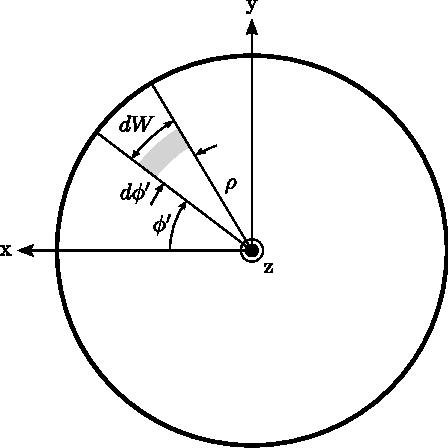
\includegraphics[scale = 1]{Figures/Principios/principios_5.pdf}}
\subfigure[Vista lateral.]{
\label{fig_principios:6}
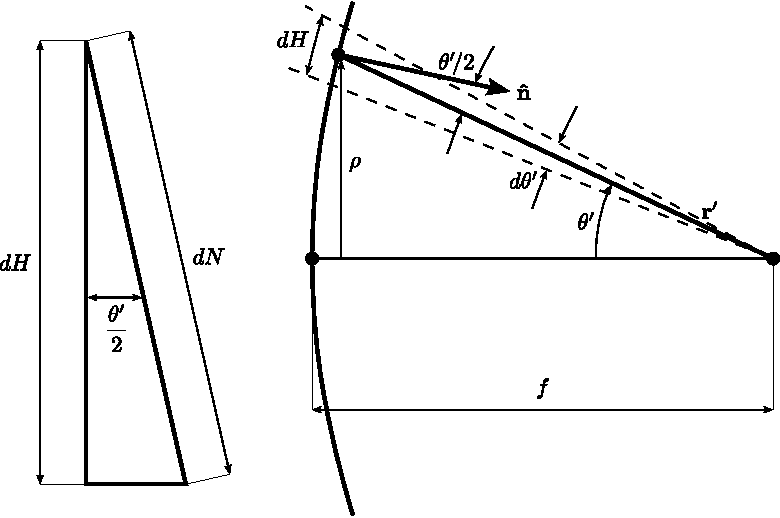
\includegraphics[scale = 1]{Figures/Principios/principios_6.pdf}}
\caption{Proyección del área y vista lateral del reflector.}
\label{grup_fig_principios:1}
\end{figure}
%%%%
De acuerdo a la geometría de la figura \ref{grup_fig_principios:1}:
%%%%
\begin{align}
ds' = dWdN = \left(r'\sen\theta 'd\phi '\right)\!\left[r'\sec\left(\frac{\theta '}{2}\right)\!d\theta '\right] = {r'}^2\sen\theta '\sec\left(\frac{\theta '}{2}\right)\!d\theta 'd\phi '
\label{ec_principios:48}
\end{align}
%%%%
donde:
%%%%%
\begin{align}
dW &= r'\sen\theta 'd\phi'
\tag{\ref{ec_principios:48}a}
\label{ec_principios:49}\\
\begin{split}
dH &= -\versor{r}\prodesc d\mathbf{N} = -\versor{r}\prodesc\versor{n}\,dN\\
&= -\versor{r}\prodesc\left[-\cos\left(\frac{\theta '}{2}\right)\!\versor{r} + \sen\left(\frac{\theta '}{2}\right)\!\versor{\uptheta}\right]\!dN = \cos\left(\frac{\theta '}{2}\right)\!dN
\end{split}
\tag{\ref{ec_principios:48}b}
\label{ec_principios:50}\\
dN &= \sec\left(\frac{\theta '}{2}\right)\!dH = \sec\left(\frac{\theta '}{2}\right)\!r'd\theta ' = r'\sec\left(\frac{\theta '}{2}\right)\!d\theta '
\tag{\ref{ec_principios:48}c}
\label{ec_principios:51}
\end{align}
%%%%
Empleando las expresiones \eqref{ec_principios:2}, \eqref{grup_ec_principios:9}, \eqref{ec_principios:47} y \eqref{ec_principios:48}, las expresiones de los campos \eqref{grup_ec_principios:7} quedan reducidas a:
%%%%
\begin{subequations}
\label{grup_ec_principios:10}
\begin{align}
E_{\theta} &= -j\frac{\omega\mu FC_1}{2\eta\pi r}e^{- jkr}\left(-\cos\theta\cos\phi\,\mathbf{I}_1 + \cos\theta\sen\phi\,\mathbf{I}_2 + \sen\theta\,\mathbf{I}_3\right)
\label{ec_principios:52}\\
E_{\phi} &= -j\frac{\omega\mu FC_1}{2\eta\pi r}e^{- jkr}\left(\sen\phi\,\mathbf{I}_1 + \cos\phi\mathbf{I}_2\right)
\label{ec_principios:53}
\end{align}
\end{subequations}
%%%%
donde:
%%%%
\begin{subequations}
\label{grup_ec_principios:11}
\begin{align}
\begin{split}
\mathbf{I}_1 &= \!\!\bigint_{\phi ' = 0}^{2\pi}\!\!\bigint_{\theta ' = 0}^{\theta_0}\!\!\!\!\!\sqrt{G_f\left(\theta ',\phi '\right)}\,\dfrac{\sen^2\theta '\sen\left(\dfrac{\theta '}{2}\right)\sen\phi '\cos\phi '}{\cos^3\left(\dfrac{\theta '}{2}\right)\!\sqrt{1 - \sen^2\theta '\sen^2\phi '}}\\
&\times e^{-jkF\left[1 - \sen\theta\sen\theta '\cos\left(\phi - \phi '\right) - \cos\theta\cos\theta '\right]/\cos^2\left(\frac{\theta '}{2}\right)}d\theta 'd\phi '
\end{split}
\label{ec_principios:54}\\
\begin{split}
\mathbf{I}_2 &= \!\!\bigint_{\phi ' = 0}^{2\pi}\!\!\bigint_{\theta ' = 0}^{\theta_0}\!\!\!\!\!\sqrt{G_f\left(\theta ',\phi '\right)}\,\dfrac{\sen\theta '\left[\cos\theta '\sen^2\phi ' + \cos^2\phi '\right]}{\cos^2\left(\dfrac{\theta '}{2}\right)\!\sqrt{1 - \sen^2\theta '\sen^2\phi '}}\\
&\times e^{-jkF\left[1 - \sen\theta\sen\theta '\cos\left(\phi - \phi '\right) - \cos\theta\cos\theta '\right]/\cos^2\left(\frac{\theta '}{2}\right)}d\theta 'd\phi '
\end{split}
\label{ec_principios:55}\\
\begin{split}
\mathbf{I}_3 &= \!\!\bigint_{\phi ' = 0}^{2\pi}\!\!\bigint_{\theta ' = 0}^{\theta_0}\!\!\!\!\!\sqrt{G_f\left(\theta ',\phi '\right)}\,\dfrac{\sen\theta '\cos\theta '\sen\left(\dfrac{\theta '}{2}\right)\sen\phi '}{\cos^3\left(\dfrac{\theta '}{2}\right)\!\sqrt{1 - \sen^2\theta '\sen^2\phi '}}\\
&\times e^{-jkF\left[1 - \sen\theta\sen\theta '\cos\left(\phi - \phi '\right) - \cos\theta\cos\theta '\right]/\cos^2\left(\frac{\theta '}{2}\right)}d\theta 'd\phi '
\end{split}
\label{ec_principios:56}
\end{align}
\end{subequations}
%%%%

%%%%
\section{Ganancia y eficiencia de abertura}
\label{sec_principios_gan_ef_abertura}
%%%%

%%%%
En la sección \ref{subsec_intro_area_efec}, se dedujo que la ganancia de una antena puede expresarse como:
%%%%
\begin{align}
G_0 = \dfrac{4\pi}{\lambda^2}A_{em}
\label{ec_principios:57}
\end{align}
%%%%
y empleando la expresión \eqref{ec_intro:54}, $G_0$ queda expresada como:
%%%%
\begin{align}
G_0 = \dfrac{4\pi}{\lambda^2}\varepsilon_{ap}A_p
\label{ec_principios:58}
\end{align}
%%%%
Conociendo la longitud de onda y el área de la superficie física $A_p$, el estudio de la ganancia se reduce a la determinación de la eficiencia de abertura $\varepsilon_{ap}$, la cual puede ser expresada como:
%%%%
\begin{align}
\varepsilon_{ap} = e_r\varepsilon_t\varepsilon_s\varepsilon_o
\label{ec_principios:59}
\end{align}
%%%%
donde:
%%%%
\begin{align*}
e_r = &\text{ Eficiencia de radiación, debida a pérdidas óhmicas.}\\
\varepsilon_t = &\text{ Eficiencia\hspace{0.43mm} de\hspace{0.43mm} iluminación,\hspace{0.43mm} debida\hspace{0.43mm} a\hspace{0.43mm} la\hspace{0.43mm} distribución\hspace{0.43mm} de\hspace{0.43mm} amplitud\hspace{0.43mm} no\hspace{0.43mm} uniforme\hspace{0.43mm} del}\\
&\text{ diagrama de radiación del alimentador sobre la superficie del reflector.}\\
\varepsilon_s = &\text{ Eficiencia\hspace{0.43mm} por\hspace{0.43mm} spillover,\hspace{0.43mm} debida\hspace{0.43mm} a\hspace{0.43mm} la\hspace{0.43mm} fracción\hspace{0.43mm} de\hspace{0.43mm} la\hspace{0.43mm} potencia\hspace{0.43mm} total\hspace{0.43mm} radiada\hspace{0.43mm} por\hspace{0.43mm} el}\\
&\text{ alimentador dentro del ángulo de abertura del reflector $\theta_0$.}\\
\varepsilon_o = &\text{ Eficiencias debidas a otros factores.}
\end{align*}
%%%%
Combinando las eficiencias $\varepsilon_t$ y $\varepsilon_s$, se obtiene la \emph{eficiencia global de iluminación} $\varepsilon_i$.

%%%%
\subsection{Eficiencia global de iluminación}
\label{subsec_principios_efi_glo_ilu}
%%%%

La expresión de la eficiencia de iluminación $\varepsilon_t$ fue deducida previamente en la sección \ref{sec_fundamentos_area_ef_ant_aber}. Para un reflector parabólico de radio $a$, la expresión \eqref{ec_fundamentos:94} se reduce a:
%%%%
\begin{align}
\varepsilon_t  = \dfrac{1}{\pi a^2}\dfrac{\left|\displaystyle\int_0^{2\pi}\!\!\!\int_0^a\lvert\mathbf{E}_a\rvert\, ds'\right|^2}{\displaystyle\int_0^{2\pi}\!\!\!\int_0^a\lvert\mathbf{E}_a\rvert^2 ds'}
\label{ec_principios:60}
\end{align}
%%%%
La potencia radiada por el alimentador dentro del ángulo sólido $d\Omega ' = \sen\theta 'd\theta 'd\phi '$ debe ser igual a la potencia incidente sobre el reflector parabólico que se propaga paralela al eje \emph{z} a través de la superficie $ds' = \rho 'd\rho 'd\phi '$ \cite{Orfanidis}. Dado que $ \lvert\mathbf{E_a}\rvert ^2/2\eta$ es la densidad de potencia del campo sobre la abertura y asumiendo que $U_f\left(\theta ',\phi '\right)$ es la intensidad de radiación del alimentador, a partir de las condiciones de potencia surge la relación:
%%%%
\begin{align}
\dfrac{1}{2\eta}\lvert\mathbf{E_a}\rvert ^2ds' = U_f\left(\theta ',\phi '\right)\!d\Omega '\Longrightarrow \dfrac{1}{2\eta}\lvert\mathbf{E_a}\rvert ^2\rho 'd\rho ' = U_f\left(\theta ',\phi '\right)\sen\theta 'd\theta '
\label{ec_principios:61}
\end{align}
%%%%
Derivando la expresión \eqref{ec_principios:3}, se obtiene:
%%%%
\begin{align}
\dfrac{d\rho '}{d\theta '} = \dfrac{F}{\cos^2\theta '}
\label{ec_principios:62}
\end{align}
%%%%
y empleando las expresiones \eqref{ec_principios:2} y \eqref{ec_principios:62}, se llega a:
%%%%
\begin{align}
d\rho ' = r'd\theta '
\label{ec_principios:63}
\end{align}
%%%%
A partir de las expresiones \eqref{ec_principios:3} y \eqref{ec_principios:63}, se obtiene:
%%%%
\begin{align}
\rho 'd\rho ' = {r'}^2\sen\theta 'd\theta ' = r'2F\tan\left(\frac{\theta '}{2}\right)d\theta '
\label{ec_principios:64}
\end{align}
%%%%
Empleando las expresiones \eqref{ec_principios:61} y \eqref{ec_principios:64}, se obtienen las relaciones:
%%%%
\begin{subequations}
\label{grup_ec_principios:12}
\begin{align}
\lvert\mathbf{E_a}\rvert ^2 &= \dfrac{2\eta\,U_f\left(\theta ',\phi '\right)}{{r'}^2}
\label{ec_principios:65}\\
\lvert\mathbf{E_a}\rvert &= \dfrac{\sqrt{2\eta\,U_f\left(\theta ',\phi '\right)}}{r'}
\label{ec_principios:66}
\end{align}
\end{subequations}
%%%%
y relacionando las expresiones \eqref{ec_principios:64} y \eqref{grup_ec_principios:12}, se llega a:
%%%%
\begin{subequations}
\label{grup_ec_principios:13}
\begin{align}
\lvert\mathbf{E_a}\rvert ^2ds' &= \lvert\mathbf{E_a}\rvert ^2\rho 'd\rho 'd\phi ' = 2\eta\,U_f\left(\theta ',\phi '\right)\sen\theta 'd\theta 'd\phi '
\label{ec_principios:67}\\
\lvert\mathbf{E_a}\rvert ds' &= \lvert\mathbf{E_a}\rvert \rho 'd\rho 'd\phi ' = 2F\sqrt{2\eta\,U_f\left(\theta ',\phi '\right)}\tan\left(\frac{\theta '}{2}\right)\!d\theta 'd\phi '
\label{ec_principios:68}
\end{align}
\end{subequations}
%%%%
Empleando las expresiones \eqref{ec_principios:60} y \eqref{grup_ec_principios:13}, la eficiencia de iluminación queda expresada como:
%%%%
\begin{align}
\varepsilon_t  = \dfrac{4F^2}{\pi a^2}\dfrac{\left|\displaystyle\int_0^{2\pi}\!\!\!\int_0^{\theta_0}\! \sqrt{\,U_f\left(\theta ',\phi '\right)}\tan\left(\frac{\theta '}{2}\right)\!d\theta 'd\phi '\right|^2}{\displaystyle\int_0^{2\pi}\!\!\!\int_0^{\theta_0}U_f\left(\theta ',\phi '\right)\sen\theta 'd\theta 'd\phi '}
\label{ec_principios:69}
\end{align}
%%%%
Considerando que $a = D/2$ y normalizando la intensidad de radiación del alimentador $U_f$, la expresión \eqref{ec_principios:69} se reduce a:
%%%%
\begin{align}
\varepsilon_t  = \dfrac{16F^2}{\pi D^2}\dfrac{\left|\displaystyle\int_0^{2\pi}\!\!\!\int_0^{\theta_0}\! \sqrt{\,F_{nf}\left(\theta ',\phi '\right)}\tan\left(\frac{\theta '}{2}\right)\!d\theta 'd\phi '\right|^2}{\displaystyle\int_0^{2\pi}\!\!\!\int_0^{\theta_0}F_{nf}\left(\theta ',\phi '\right)\sen\theta 'd\theta 'd\phi '}
\label{ec_principios:70}
\end{align}
%%%%
donde $F_{nf}$ es el factor de diagrama de potencia normalizado del alimentador, cuya relación con la intensidad de radiación fue deducida en la sección \ref{subsec_intro_direc}.

Finalmente, introduciendo la expresión \eqref{ec_principios:4}, $\varepsilon_t$ queda expresada como:
%%%%
\begin{align}
\varepsilon_t  = \dfrac{1}{\pi}\cot^2\left(\frac{\theta_0}{2}\right)\dfrac{\left|\displaystyle\int_0^{2\pi}\!\!\!\int_0^{\theta_0}\! \sqrt{\,F_{nf}\left(\theta ',\phi '\right)}\tan\left(\frac{\theta '}{2}\right)\!d\theta 'd\phi '\right|^2}{\displaystyle\int_0^{2\pi}\!\!\!\int_0^{\theta_0}F_{nf}\left(\theta ',\phi '\right)\sen\theta 'd\theta 'd\phi '}
\label{ec_principios:71}
\end{align}
%%%%
Por definición, la eficiencia por spillover $\varepsilon_s$ es la relación entre la potencia captada por el reflector respecto a la potencia total radiada por el alimentador, por lo que puede expresarse como:
%%%%
\begin{align}
\varepsilon_s  = \dfrac{\displaystyle\int_0^{2\pi}\!\!\!\int_0^{\theta_0}F_{nf}\left(\theta ',\phi '\right)\sen\theta 'd\theta 'd\phi '}{\displaystyle\int_0^{2\pi}\!\!\!\int_0^{\pi}F_{nf}\left(\theta ',\phi '\right)\sen\theta 'd\theta 'd\phi '}
\label{ec_principios:72}
\end{align}
%%%%
Combinando las eficiencias $\varepsilon_t$ y $\varepsilon_s$ y asumiendo condiciones ideales en las que no existen pérdidas óhmicas ($e_r = 1$) y debidas a otros factores ($\varepsilon_o = 1$), la eficiencia de abertura $\varepsilon_{ap}$ queda expresada como:
%%%%
\begin{align}
\varepsilon_{ap}  = \varepsilon_i = \varepsilon_t\varepsilon_s = \dfrac{1}{\pi}\cot^2\left(\frac{\theta_0}{2}\right)\dfrac{\left|\displaystyle\int_0^{2\pi}\!\!\!\int_0^{\theta_0}\! \sqrt{\,F_{nf}\left(\theta ',\phi '\right)}\tan\left(\frac{\theta '}{2}\right)\!d\theta 'd\phi '\right|^2}{\displaystyle\int_0^{2\pi}\!\!\!\int_0^{\pi}F_{nf}\left(\theta ',\phi '\right)\sen\theta 'd\theta 'd\phi '}
\label{ec_principios:73}
\end{align}
%%%%
donde $\varepsilon_i$ es la \emph{eficiencia global de iluminación}.

Empleando las expresiones \eqref{ec_intro:20} - \eqref{ec_intro:22}, la expresión \eqref{ec_principios:73} se reduce a:
%%%%
\begin{align}
\varepsilon_{ap}  = \dfrac{1}{4\pi ^2}\cot^2\left(\frac{\theta_0}{2}\right)\left|\displaystyle\int_0^{2\pi}\!\!\!\int_0^{\theta_0}\! \sqrt{\,G_f\left(\theta ',\phi '\right)}\tan\left(\frac{\theta '}{2}\right)\!d\theta 'd\phi '\right|^2
\label{ec_principios:74}
\end{align}
%%%%
donde $G_f$ es la ganancia del alimentador. Con el fin de facilitar el análisis de la eficiencia de abertura, se asume que el diagrama de radiación del alimentador posee simetría rotacional (o sea, no es función del ángulo $\upphi$'), por lo que la expresión \eqref{ec_principios:74} queda reducida a:
%%%%
\begin{align}
\varepsilon_{ap}  = \cot^2\left(\frac{\theta_0}{2}\right)\left|\displaystyle\int_0^{\theta_0}\! \sqrt{\,G_f\left(\theta '\right)}\tan\left(\frac{\theta '}{2}\right)\!d\theta '\right|^2
\label{ec_principios:75}
\end{align}
%%%%
Para lograr la máxima eficiencia de abertura, el diagrama de radiación del alimentador debería ser como el de la figura \ref{fig_principios:7}. Puede observarse que la radiación está concentrada dentro del ángulo de abertura $\theta_0$, cayendo abruptamente fuera de dicho ángulo, logrando así una $\epsilon_s = 1$. A la vez, la radiación es mayor en el ángulo $\theta_0$ que en dirección hacia el vértice del reflector, logrando así una iluminación uniforme sobre la superficie del reflector y obteniendo una $\epsilon_t = 1$. Sin embargo, los diagramas de radiación obtenidos en la práctica son más similares a los de la figura \ref{fig_principios:8}.
%%%%
\begin{figure} [H]
\centering 
\subfigure[Alimentador ideal.]{
\label{fig_principios:7}
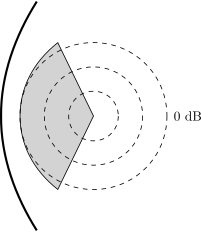
\includegraphics[scale = 1]{Figures/Principios/principios_7}}
\hspace{5mm}
\subfigure[Alimentador real.]{
\label{fig_principios:8}
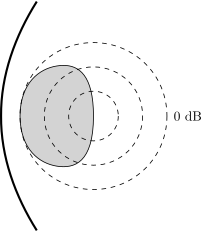
\includegraphics[scale = 1]{Figures/Principios/principios_8}}
\caption{Diagramas de radiación de alimentadores.}
\label{grup_fig_principios:2}
\end{figure}
%%%%
Cualquier alimentador en la práctica producirá pérdidas por \emph{iluminación no uniforme} y por \emph{spillover}, como puede verse en la figura \ref{fig_principios:9}. Un diagrama de radiación más delgado mejora $\epsilon_s$ pero empeora $\epsilon_t$, mientras que uno más ancho mejora $\epsilon_t$ pero empeora $\epsilon_s$.
%%%%
\begin{figure}[H]
\centering
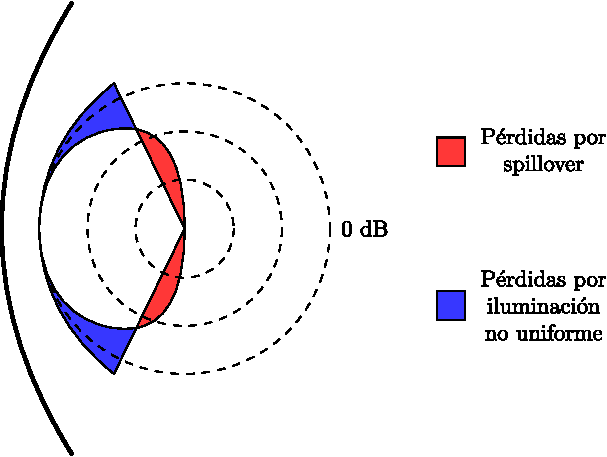
\includegraphics[scale = 01]{Figures/Principios/principios_9}
\caption{Pérdidas en la iluminación de un reflector parabólico.}
\label{fig_principios:9}
\end{figure}
%%%%
\emph{El problema del diseño del alimentador se reduce entonces a una solución de compromiso que permita obtener una} $\epsilon_s$ \emph{y una} $\epsilon_t$ \emph{tales que la eficiencia de abertura} $\epsilon_{ap}$ \emph{sea máxima}.

Para demostrar la variación de la eficiencia de abertura en función del ángulo $\theta_0$ y de la relación $F/D$, Silver \cite{Silver} consideró un tipo de alimentador cuyo diagrama de radiación está definido por:
%%%%
\begin{align}
G_f\left(\theta '\right) = 
\begin{cases} 
{G_0}^{\left(n\right)}\cos^n\left(\theta '\right)  &\mbox{si}\;0\leq\theta '\leq\pi/2\\
0  &\text{si}\;\pi/2\leq\theta '\leq\pi
\end{cases}
\label{ec_principios:76}
\end{align}
%%%%
donde ${G_0}^{\left(n\right)}$ es una constante dada por el valor $n$. Aunque son ideales, estos diagramas de radiación se escogieron porque permiten obtener expresiones cerradas y porque generalmente permiten obtener una buena representación del lóbulo principal en la práctica. La radiación directa del alimentador ($\uptheta$' $> \pi/2$) se asume nula con el fin de evitar la interferencia con la radiación reflejada.

A partir de la relación:
%%%%
\begin{align}
\iint\limits_{S}G_f\left(\theta '\right)\!d\Omega ' = \iint\limits_{S}G_f\left(\theta '\right)\sen\theta 'd\theta 'd\phi ' = 4\pi
\label{ec_principios:77}
\end{align}
%%%%
se determina la constante ${G_0}^{\left(n\right)}$:
%%%%
\begin{align}
{G_0}^{\left(n\right)}\!\int_0^{\,\pi /2}\!\cos^n\theta '\sen\theta 'd\theta ' = 2 \Longrightarrow {G_0}^{\left(n\right)} = 2\left(n + 1\right)
\label{ec_principios:78}
\end{align}
%%%%
por lo que la expresión \eqref{ec_principios:76} se reduce a:
%%%%
\begin{align}
G_f\left(\theta '\right) = 
\begin{cases} 
2\left(n + 1\right)\cos^n\left(\theta '\right)  &\mbox{si}\;0\leq\theta '\leq\pi/2\\
0  &\text{si}\;\pi/2\leq\theta '\leq\pi
\end{cases}
\label{ec_principios:79}
\end{align}
%%%%
La expresión \eqref{ec_principios:75}, para valores pares de $n$ comprendidos entre 2 y 8 y empleando la expresión \eqref{ec_principios:79}, resulta:
%%%%
\begin{subequations}
\label{grup_ec_principios:14}
\begin{align}
\epsilon_{ap}\left(n = 2\right) &= 24\left\{\sen^2\left(\frac{\theta_0}{2}\right) + \ln\left[\cos\left(\frac{\theta_0}{2}\right)\right]\right\}^2\!\cot^2\left(\frac{\theta_0}{2}\right)
\label{ec_principios:80}\\
\epsilon_{ap}\left(n = 4\right) &= 40\left\{\sen^4\left(\frac{\theta_0}{2}\right) + \ln\left[\cos\left(\frac{\theta_0}{2}\right)\right]\right\}^2\!\cot^2\left(\frac{\theta_0}{2}\right)
\label{ec_principios:81}\\
\epsilon_{ap}\left(n = 6\right) &= 14\left\{2\ln\left[\cos\left(\frac{\theta_0}{2}\right)\right] + \frac{\left(1 - \cos\theta_0\right)^3}{3} + \frac{1}{2}\sen^2\theta_0\right\}^2\!\cot^2\left(\frac{\theta_0}{2}\right)
\label{ec_principios:82}\\
\begin{split}
\epsilon_{ap}\left(n = 8\right) &= 18\left\{\frac{1 - \cos^4\theta_0}{4} - 2\ln\left[\cos\left(\frac{\theta_0}{2}\right)\right] - \frac{\left(1 - \cos\theta_0\right)^3}{3}\right.\\
&\left.- \frac{1}{2}\sen^2\theta_0\right\}^2\!\cot^2\left(\frac{\theta_0}{2}\right)
\end{split}
\label{ec_principios:83}
\end{align}
\end{subequations}
%%%%
Las variaciones de la eficiencia de abertura $\epsilon_{ap}$ en función del ángulo de abertura $\theta_0$ o de la relación $F/D$ para distintos valores de \emph{n} pueden verse en la figura \ref{fig_principios:10}.
%%%%
\begin{figure}[H]
\centering
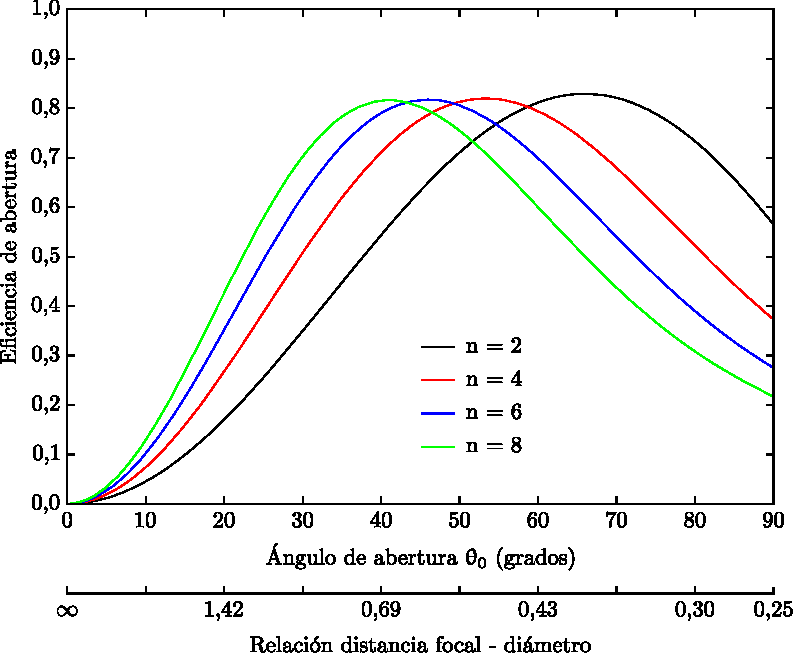
\includegraphics[scale = 0.98]{Figures/Principios/principios_10}
\caption{Eficiencia de abertura en función del ángulo $\theta_0$ (o de la relación $F/D$).}
\label{fig_principios:10}
\end{figure}
%%%%
Valiéndose de la figura \ref{fig_principios:11}, para cada valor de $n$ se analiza la diferencia entre las potencias incidentes en el borde y el vértice del reflector $EI$, cuya expresión es:
%%%%
\begin{align}
EI_{dB} = 10\log\left(G_{fn}\left(\theta_0\right)\right) + P\!A
\label{ec_principios:84}
\end{align}
%%%%
donde $G_{fn}\left(\theta '\right)$ corresponde a la ganancia normalizada del alimentador dado por la expresión \eqref{ec_principios:79} y $P\!A$ es la atenuación en el espacio libre producida en la diferencia de caminos $\Delta r$ que se expresa como:
%%%%
\begin{align}
P\!A_{dB} = 20\log\left(\dfrac{F}{r_0}\right)
\label{ec_principios:85}
\end{align}
%%%%
\begin{figure}[H]
\centering
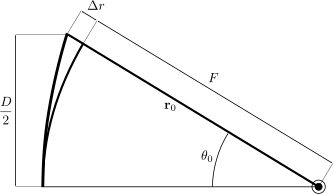
\includegraphics[scale = 1]{Figures/Principios/principios_11}
\caption{Iluminación en el borde y en el vértice del reflector.}
\label{fig_principios:11}
\end{figure}
%%%%
Aplicando propiedades trigonométricas, la expresión \eqref{ec_principios:85} se reduce a:
%%%%
\begin{align}
P\!A_{dB} = 20\log\left(2\,\dfrac{F}{D}\sen\theta_0\right)
\label{ec_principios:86}
\end{align}
%%%%
En la tabla \ref{tabla_principios:1} pueden observarse los resultados obtenidos para los valores de $n$ comprendidos entre 2 y 8.
%%%%
\begin{table}[H]
\centering
\begin{tabular}{|c|c|c|c|c|c|c|c|c|}
\hline
n & $\epsilon_s$ & $\epsilon_t$ & $\epsilon_{ap}$ & $\theta_0\,$(grados) & $F/D$ & $G_{fn}\left(\theta_0\right)\,$(dB) & $P\!A\,$(dB) & $EI\,$(dB)\\
\hline
2 & 0,933 & 0,889 & 0,829 & 60,0 & 0,385 & -7,810 & -3,055 & -10,865\\
\hline
4 & 0,924 & 0,887 & 0,820 & 53,3 & 0,498 & -8,946 & -1,952 & -10,898\\
\hline
6 & 0,921 & 0,887 & 0,817 & 45,9 & 0,590 & -9,470 & -1,436 & -10,906\\
\hline
8 & 0,920 & 0,887 & 0,816 & 41,0 & 0,669 & -9,772 & -1,136 & -10,908\\
\hline
\end{tabular}
\caption{Eficiencias de abertura y diferencias entre las potencias incidentes en el borde y el vértice del reflector para distintos valores de $n$.}
\label{tabla_principios:1}
\end{table}
%%%%
Los valores de $EI$ para los casos analizados son aproximadamente -11 dB, y la eficiencia de abertura se encuentra en torno al 82 \%. Entonces, puede decirse que \emph{la eficiencia de abertura en términos de iluminación es máxima cuando la diferencia entre las potencias incidentes en el borde y en el vértice del reflector es de -11 dB}. Esta es la solución de compromiso a partir de la cual se debe diseñar el alimentador.

%%%%
\subsection{Otras eficiencias}
\label{subsec_principios_otras_efi}
%%%%

La eficiencia de abertura se debe, además de al patrón de iluminación del reflector, a otros grupo de factores; se define entonces a la \emph{eficiencia debida a otros factores} $\varepsilon_o$ como:
%%%%
\begin{align*}
\varepsilon_o = \varepsilon_p\varepsilon_b\varepsilon_x
\end{align*}
%%%%
donde:
%%%%
\begin{enumerate}
\item \emph{Eficiencia de fase $\varepsilon_p$}, debida a la no uniformidad de la fase del campo sobre el plano de abertura.
\item \emph{Eficiencia por bloqueo $\varepsilon_b$}, debida al bloqueo parcial del campo reflejado producido por el alimentador.
\item \emph{Eficiencia por polarización cruzada $\varepsilon_x$}, debida a la existencia de campos con polariación cruzada sobre el plano de abertura.
\end{enumerate}
%%%%
Existen otros factores que inciden en la eficiencia de abertura, como las irregularidades en la superficie del reflector y los desplazamientos axiales y laterales del alimentador respecto de su ubicación en el foco, pero se desprecian con el fin de facilitar el estudio de $\varepsilon_{ap}$.

La expresión de la eficiencia de fase $\varepsilon_p$ fue deducida previamente en la sección \ref{sec_fundamentos_area_ef_ant_aber}. Empleando el mismo análisis utilizado para deducir la eficiencia de iluminación global $\varepsilon_i$, la expresión \eqref{ec_fundamentos:95} se reduce a:
%%%%
\begin{align}
\varepsilon_p  = \dfrac{\left|\displaystyle\int_0^{2\pi}\!\!\!\int_0^{\theta_0}\! \sqrt{\,F_{nf}\left(\theta ',\phi '\right)}\,e^{-jk\delta}\tan\left(\frac{\theta '}{2}\right)\!d\theta 'd\phi '\right|^2}{\left|\displaystyle\int_0^{2\pi}\!\!\!\int_0^{\theta_0}\! \sqrt{\,F_{nf}\left(\theta ',\phi '\right)}\tan\left(\frac{\theta '}{2}\right)\!d\theta 'd\phi '\right|^2}
\label{ec_principios:87}
\end{align}
%%%%
donde el término $e^{-jk\delta}$ representa la variación de fase de los campos sobre el plano de abertura, y $\delta$ depende directamente de las características de radiación del alimentador.

En la sección \ref{sec_principios_intro} se determinó que si el centro de fase del alimentador coincide con el foco del reflector parabólico, la fase a través del plano de abertura será uniforme. Entonces, \emph{una característica deseable del alimentador es que su centro de fase coincida con el foco del reflector}, en cuyo caso $\delta = 0$ y la eficiencia de fase $\varepsilon_p = 1$. Muchas veces no es posible obtener un alimentador que cumpla tal característica; en tal caso, el alimentador tendrá un cierto \emph{error de fase}, el cual deberá ser lo menor posible para que $\varepsilon_p$ sea máxima.

La eficiencia por bloqueo $\varepsilon_b$ depende directamente de las dimensiones del alimentador, y puede determinarse aproximadamente a partir de la expresión \cite{Stutzman}:
%%%%
\begin{align}
\varepsilon_b  = \left(1 - \dfrac{1}{\varepsilon_t}\dfrac{A_f}{A_p}\right)^2
\label{ec_principios:88}
\end{align}
%%%%
donde $A_f$ es el área de bloqueo proyectada por el alimentador y $A_p$ es el área proyectada del reflector parabólico.

Dado que en la medida que se incrementen las dimensiones del alimentador disminuye $\varepsilon_b$, \emph{otra característica deseable del alimentador es que sus dimensiones sean lo menor posible}.

La eficiencia por polarización cruzada $\varepsilon_x$ se debe a contribuciones del alimentador, ya que los reflectores parabólicos de foco centrado no introducen componentes contrapolares. La mayoría de las veces puede despreciarse, fundamentalmente considerando que la polarización cruzada es prácticamente nula en la dirección de propagación principal $\left(\uptheta = 0^{\circ}\right)$. En la sección \ref{sec_polarizacion_cruzada} se analizará más en detalle la polarización cruzada generada por una antena parabólica.

%%%%
\section{Polarización cruzada}
\label{sec_polarizacion_cruzada}
%%%%

Para el estudio de la polarización cruzada en un reflector parabólico, se considera inicialmente que el alimentador está linealmente polarizado a lo largo del eje \emph{y}. Si el diagrama de radiación del alimentador tuviera simetría rotacional, es decir, si fuera solamente función de $\uptheta$' y no de $\upphi$', la componente contrapolar de los campos radiados por el reflector parabólico sería nula. Puede decirse entonces que en una antena parabólica de foco centrado \emph{la existencia de componentes contrapolares del campo se debe exclusivamente a contribuciones del alimentador} \cite{Stutzman}.

Es deseable, por lo tanto, que un alimentador tenga las siguientes características:
\begin{itemize}
\item Baja polarización cruzada.
\item Diagrama de radiación con la mayor simetría rotacional posible.
\end{itemize}
%%%%
A partir de los campos radiados por el reflector \eqref{grup_ec_principios:10}, se determinan las componentes $E_x$ y $E_y$, donde $E_y$ corresponde a la copolarización y $E_x$ a la polarización cruzada. La componente contrapolar es nula para los planos \emph{E} ($\upphi = 90^{\circ}$) y \emph{H} ($\upphi = 0^{\circ}$) y máxima para el plano $\upphi = 45^{\circ}$; además, disminuye en la medida que la relación $F/D$ aumente \cite{Stutzman} \cite{Collin}. En la figura \ref{fig_principios:12} puede observarse como varía comúnmente la copolarización y la polarización cruzada de una antena parabólica de foco centrado en función del ángulo $\uptheta$, para el plano $\upphi = 45^{\circ}$.
%%%%
\begin{figure}[H]
\centering
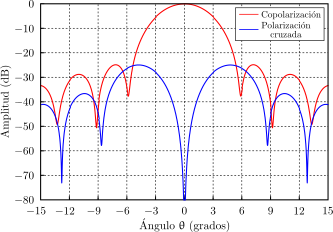
\includegraphics[scale = 1]{Figures/Principios/principios_12}
\caption{Copolarización y polarización cruzada de una antena parabólica de foco centrado, para el plano $\upphi = 45^{\circ}$.}
\label{fig_principios:12}
\end{figure}
%%%%